\documentclass[a4paper,12pt]{report}
\usepackage[utf8]{inputenc}
\usepackage{mathtools}
\usepackage{listings}
\usepackage{framed}
\usepackage{epstopdf}
\usepackage[spanish]{babel}
\usepackage{appendix}
\usepackage[usenames,dvipsnames,table]{xcolor}
\usepackage{minted}
\usepackage[a4paper]{geometry}

\newminted{vhdl}{mathescape, linenos, numbersep=15pt, frame=lines,framesep=2mm}
               
\newminted{matlab}{mathescape, linenos, numbersep=15pt, frame=lines,framesep=2mm}               

\definecolor{bg}{rgb}{0.95,0.95,0.95}


% Allow the change of line spacing
\usepackage{setspace}
\usepackage{tabularx}
\usepackage{graphicx}


%\usepackage{hyperref}
%\usepackage{breakurl}

%opening
%\title{Trainmining}
%\author{Grupo de Sistemas Inteligentes \\ Universidad Politécnica de Madrid}


\begin{document}
\newcommand\litem[1]{\item{\bfseries #1 }}
\renewcommand{\arraystretch}{1.5} %Makes tables less crammed

\newcommand\headcell[1]{%
  \multicolumn{1}{c|}{\cellcolor{MidnightBlue}\bfseries\sffamily\textcolor{white}{#1}}
}
\newcommand\headcelld[1]{%
  \multicolumn{1}{c||}{\cellcolor{MidnightBlue}\bfseries\sffamily\textcolor{white}{#1}}
}

%\renewcommand{\abstractname}{Executive Summary}
%\begin{abstract}
%
%\end{abstract}

% Set line spacing to 1.5
%\onehalfspacing

% Begin a new titlepage. Tit	lepages have special settings like the absence of page numbers.
\begin{titlepage}
\sffamily
% Set the text of the page to right-aligned until \end{flushright}
\begin{flushright}

% Set the space between right page border and text to 2.5cm
\rightskip=-0cm

% Show an image at this position 
%\includegraphics[bb=0 0 204 110]{web40logo.png}

% Skip a little space
\vspace*{3cm}


% Create a title for the document and write it in bold font
\huge{\textbf{DCSE - Grupo especial}}
% Again, do a line break
\linebreak
% Create a subtitle
\LARGE{Trabajo con herramientas de diseño CAD-VHDL.}

% Skip some space
\vspace*{10cm}




\large{Memoria del proyecto}
\linebreak
\normalsize{Madrid, Noviembre 2012}

% Skip some space
\vspace*{3cm}


% Provide some author information
\normalsize{Autor:}
\linebreak
\large{Adrián Pérez Orozco}
\linebreak

% End right-alignment at this point
\end{flushright}
% End the title page
\end{titlepage}

%\maketitle

\newpage
\tableofcontents % indice de contenidos
\addcontentsline{toc}{chapter}{Contenidos} % para que aparezca en el indice de 

\chapter*{Introducción}
\addcontentsline{toc}{chapter}{Introducción}
\section*{Descripción del proyecto}
\addcontentsline{toc}{section}{Descripción del proyecto}
En esta memoria vamos a tratar un proyecto realizado para la asignatura \emph{Diseño de Circuitos y Sistemas Electrónicos} impartida en la ETSI de Telecomunicación de la Universidad Politécnica de Madrid.

El proyecto se propone como trabajo adicional a la asignatura, para tratar los temas de diseño de circuitos digitales de una forma más práctica y obtener conocimientos mucho más amplios sobre tecnologías relacionadas con estos campos.

En concreto, la propuesta consiste en el diseño y simulación de un sistema utilizando VHDL. El sistema propuesto consiste en un ecualizador de audio, del cual se implementarán algunos subsistemas de procesado digital en VHDL. Esta práctica se apoya sobre el trabajo realizado en el año anterior en el \emph{Laboratorio de Sistemas Electrónicos Digitales}, donde se realizó este sistema utilizando un microcontrolador.

El esquema de dicho sistema puede verse en la figura~\ref{fig:sysdesc}. El proyecto que nos ocupa se centrará en la realización del subsistema de procesado digital de audio, cuyo esquema puede verse en la figura~\ref{fig:digproc}.

El proyecto se ha estructurado en 5 hitos, correspondientes al diseño de cada uno de los subsistemas necesarios, de la forma siguiente:

\begin{description}
\item[Hito 1] Diseño y caracterización de filtros
\item[Hito 2] Subsistema de ecualización
\item[Hito 3] Reverberación
\item[Hito 4] Integración global
\item[Hito 5] Mejoras
\end{description}

Además, se propone un \emph{hito 0} de introducción a VHDL, con el objetivo de familiarizarse con el lenguaje VHDL y las herramientas que se utilizarán para el desarrollo y simulación del sistema.

Para la realización del proyecto se utilizará la herramienta ModelSim. De forma auxiliar, se utilizará la herramienta MATLAB para obtener de forma más sencilla y eficiente información sobre las respuestas de los filtros tanto en el tiempo como en el dominio de la frecuencia.

\begin{figure}[hbt]
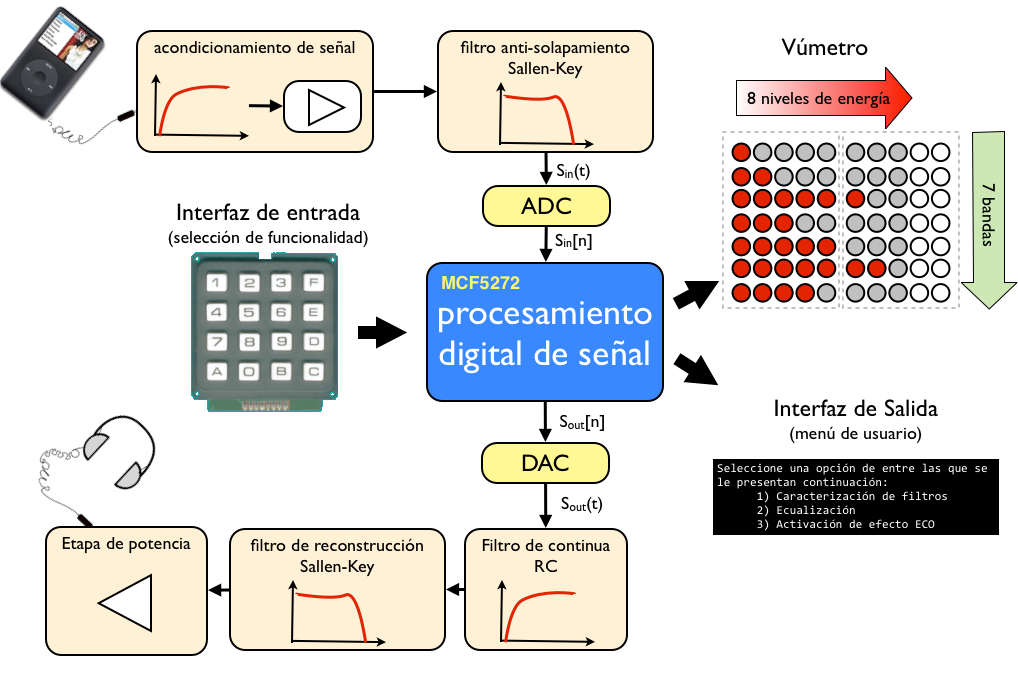
\includegraphics[width=\textwidth]{img/system_description.png} 
\caption{Descripcción del sistema completo} \label{fig:sysdesc}
\end{figure}

\begin{figure}[hbt]
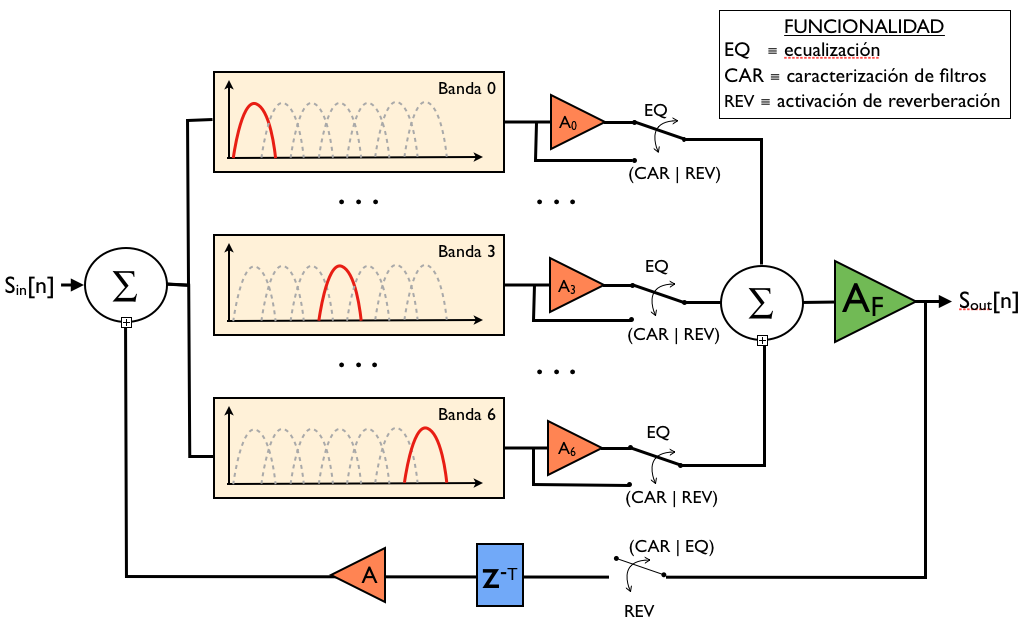
\includegraphics[width=\textwidth]{img/digital_proc.png} 
\caption{Descripcción del subsistema de procesado digital} \label{fig:digproc}
\end{figure}

\chapter{Diseño y caracterización de filtros}
En este capítulo vamos a detallar el proceso de diseño y caracterización de los filtros digitales, lo que corresponde al Hito 1 de nuestro proyecto.

\section{Descripción de filtros para las distintas bandas de frecuencias}
El sistema propuesto se trata de un ecualizador de audio, por lo que las señales de entrada que tendremos estarán comprendidas en el rango de frecuencias audibles por el hombre. En concreto, la especificación del sistema propuesto propone señales cuya frecuencia estará comprendida aproximadamente entre los 22 Hz y los 2.8 KHz.

Este rango de frecuencias se dividirá en 7 bandas, para lo cual utilizaremos filtros IIR de segundo orden. Las bandas de frecuencias se detallan en la tabla \ref{tab:filters}, y los coeficientes para la realización de los filtros IIR en la tabla \ref{tab:filters}.

\begin{table}
\begin{center}
 \begin{tabular}{|c||c|c|c|}
\hline 

\headcelld{Banda} & \headcell{$f_0$} & \headcell{$f_{c1}$} & \headcell{$f_{c2}$} \\ 
\hline
\hline 
0 & 31.25 & 22.10 & 44.19 \\ 
\hline 
1 & 62.5 & 44.19 & 88.39 \\ 
\hline 
2 & 125 & 88.39 & 176.78 \\ 
\hline 
3 & 250 & 176.78 & 353.55 \\ 
\hline 
4 & 500 & 323.55 & 704.11 \\ 
\hline 
5 & 1000 & 707.11 & 1414.21 \\ 
\hline 
6 & 2000 & 1414.21 & 2828.43 \\ 
\hline 
\end{tabular} 
\caption{Descripción de las distintas bandas y sus filtros asociados} \label{tab:bands}
\end{center}
\end{table}

\begin{table}
\begin{center}
 \begin{tabular}{|c||c||c|c|c||c|c|c|}
\headcelld{Filtro} & \headcelld{Ganancia} & \headcell{$a_0$} & \headcell{$a_1$} & \headcelld{$a_2$} & \headcell{$b_0$} & \headcell{$b_1$} & \headcell{$b_2$} \\ 
\hline
\hline 
0 & 8 & 1024 & -2029 & 1006 & 1024 & 0 & -1024  \\ 
\hline 
1 & 17 & 1024 & -2011 & 988 & 1024 & 0 & -1024 \\ 
\hline 
2 & 34 & 1024 & -1970 & 955 & 1024 & 0 & -1024 \\ 
\hline 
3 & 66 & 1024 & -1878 & 890 & 1024 & 0 & -1024 \\ 
\hline 
4 & 125 & 1024 & -1660 & 772 & 1024 & 0 & -1024 \\ 
\hline 
5 & 227 & 1024 & -1115 & 569 & 1024 & 0 & -1024 \\ 
\hline 
6 & 392 & 1024 & 141 & 239 & 1024 & 0 & -1024 \\ 
\hline 
\end{tabular} 
\caption{Descripción de los coeficientes de los filtros IIR} \label{tab:filters}
\end{center}
\end{table}

\section{Implementación de los filtros en VHDL}
Para una implementación más sencilla de los filtros, utilizaremos la \emph{Forma directa II}. El detalle de esta implementación se puede ver en la figura \ref{fig:filter_diagram}.

\begin{figure}[hbt]
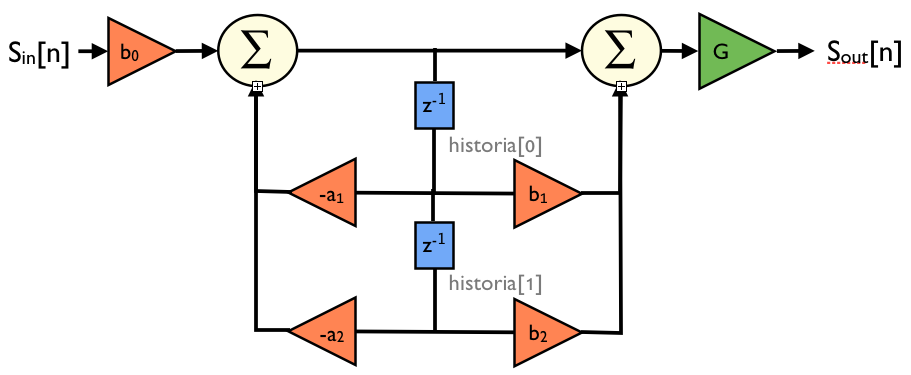
\includegraphics[width=\textwidth]{img/filter.png} 
\caption{Diagrama de bloques de un filtro IIR de segundo orden} \label{fig:filter_diagram}
\end{figure}

A la hora de implementar estos filtros digitales, tenemos que tener en cuenta una limitación muy importante. Debemos definir un ancho de palabra fijo para la representación de las señales de entrada y de salida. En nuestro caso, hemos escogido un ancho de palabra de \emph{16 bits}, correspondientes a \emph{6 bits enteros} y \emph{10 bits fraccionarios}. Esto es especialmente conveniente a la hora de representar los coeficientes de los filtros, ya que para todos ellos tenemos que $a_0 = 1024$. Normalizar los coeficientes realizando una división por 1024 equivale a desplazar los bits 10 lugares a la derecha (o lo que es lo mismo, la coma decimal 10 lugares a la izquierda). De esta forma, cuando representemos los coeficientes enteros como palabras binarias de 16 bits, bastará como tomar los 10 bits menos significativos como fraccionarios para tener el coeficiente normalizado a 1024.

A continuación se muestra el código de la implementación de los filtros en VHDL. La implementación de los 7 filtros es idéntica, cambiando únicamente el valor de las constantes $a_1$, $a_2$ y G, ya que el resto de coeficientes son iguales en todos los casos.

\begin{vhdlcode}
library ieee;
use ieee.std_logic_1164.all;
use ieee.std_logic_arith.all;
use ieee.std_logic_signed.all;

entity filterX is
port (
    sin : in std_logic_vector (15 downto 0);
    sout : out std_logic_vector (15 downto 0);
    clk : in bit);
end;

architecture filterarchX of filterX is
    signal historia0 : std_logic_vector (15 downto 0) 
                := conv_std_logic_vector(0,16);
    signal historia1 : std_logic_vector (15 downto 0) 
                := conv_std_logic_vector(0,16);
    constant b0 : std_logic_vector (15 downto 0) 
                := conv_std_logic_vector(XXX,16);
    constant b1 : std_logic_vector (15 downto 0) 
                := conv_std_logic_vector(XXX,16);
    constant b2 : std_logic_vector (15 downto 0) 
                := conv_std_logic_vector(XXX,16);
    constant a1 : std_logic_vector (15 downto 0) 
                := conv_std_logic_vector(XXX,16);
    constant a2 : std_logic_vector (15 downto 0) 
                := conv_std_logic_vector(XXX,16);
    constant gs : std_logic_vector (15 downto 0) 
                := conv_std_logic_vector(XXX,16);

begin
    filter_proc: process(clk)
        variable sum1 : std_logic_vector (31 downto 0);
        variable sum2 : std_logic_vector (31 downto 0);
        variable mult : std_logic_vector (31 downto 0);

    begin
        if (clk'event and clk = '1') then
            sum1 := b0*sin - a1*historia0 - a2*historia1;
            sum2 := sum1 + b1*historia0 + b2*historia1;
            historia1 <= historia0;
            historia0 <= sum1(25 downto 10);
            mult := gs*sum2(25 downto 10);
            sout <= mult(25 downto 10);
        end if;
    end process;
end filterarchX;
\end{vhdlcode}
\clearpage

\section{Comprobación de la validez de los filtros}
Finalmente, tras haber implementado los 7 filtros en VHDL, debemos comprobar mediante simulación que su funcionamiento es el correcto. Para ello, nos ayudaremos de la herramienta \emph{MATLAB}, que nos permite fácilmente realizar filtros dados los coeficientes \emph{a} y \emph{b} de los que disponemos.

Para comprobar que el funcionamiento de nuestros filtros es el correcto, obtendremos sus respuestas al impulso colocando en la simulación a la entrada una función $\delta[n]$. Realizaremos la misma operación en MATLAB y comprobaremos que ambas respuestas sean iguales.

En las figuras \ref{fig:filter0}, \ref{fig:filter1}, \ref{fig:filter2}, \ref{fig:filter3}, \ref{fig:filter4}, \ref{fig:filter5} y \ref{fig:filter6} se pueden ver las comprobaciones realizadas. Para cada filtro, se ha representado: La respuesta al impulso obtenida en la simulación con ModelSim (arriba a la izquierda); la respuesta al impulso obtenida con MATLAB (arriba a la derecha); y la diferencia en valor absoluto de ambas señales (debajo).

Para todas ellas, se puede apreciar que la diferencia es de un valor cientos de veces menor que el de la señal. Esto se debe al error de cuantificación introducido al limitar nuestro sistema a palabras de 16 bits con 10 bits fraccionarios. El error se va acumulando tras las diferentes iteraciones del filtro, y se empieza a compensar cuando la respuesta al impulso es negativa y el error se produce con el signo contrario. 

\begin{figure}[hbt]
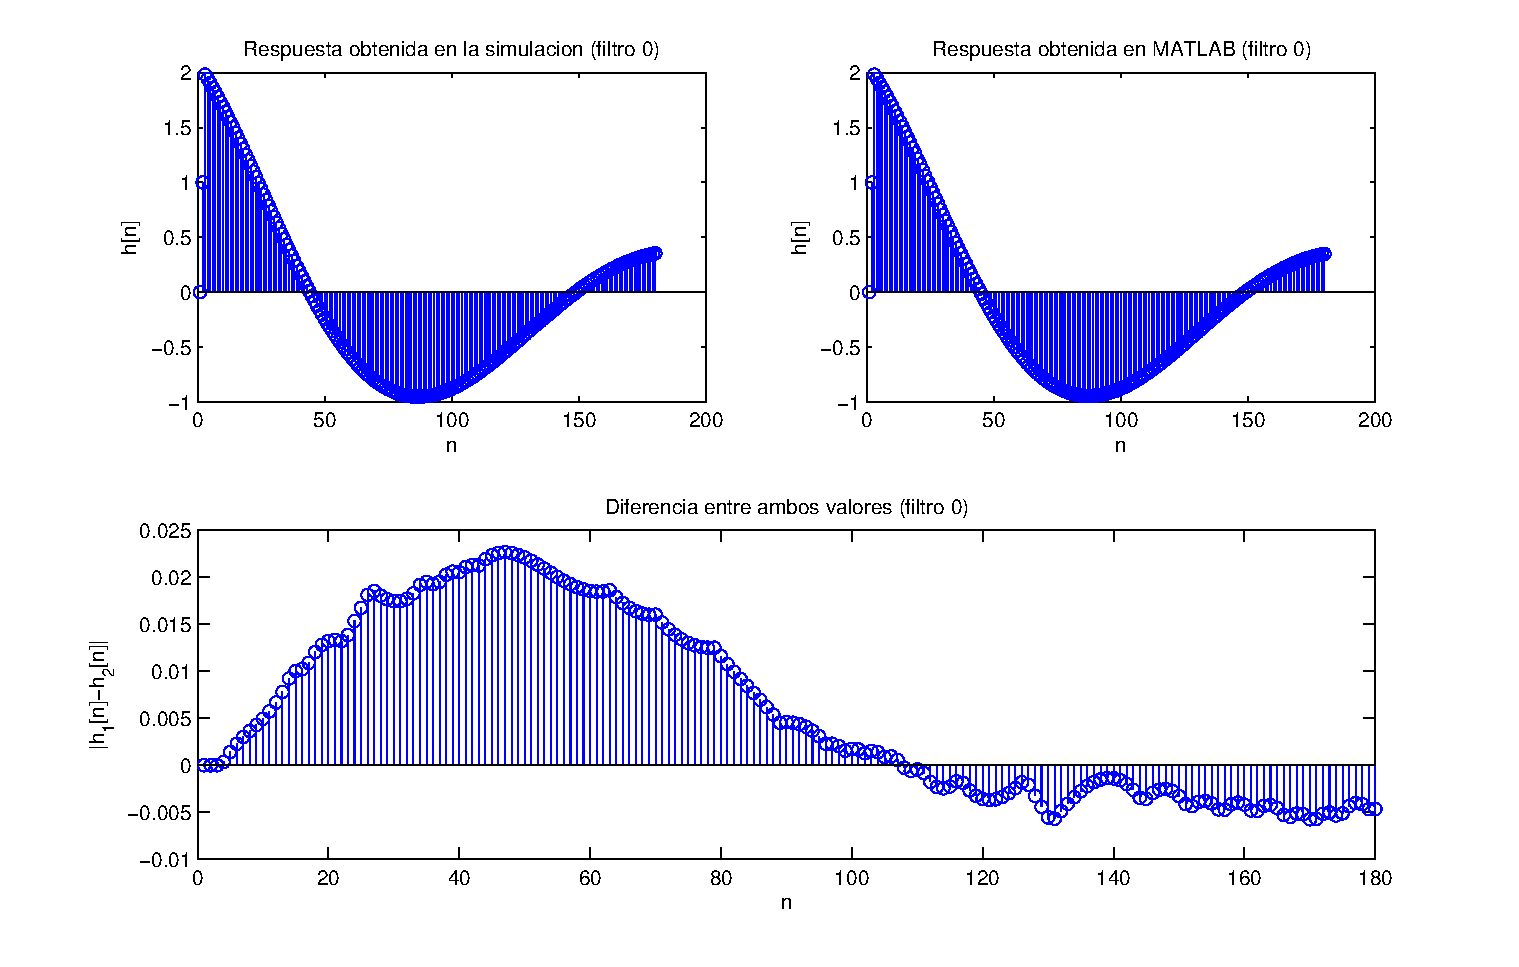
\includegraphics[width=\textwidth]{img/respfiltro0.pdf} 
\caption{Comprobación del filtro 0} \label{fig:filter0}
\end{figure}

\begin{figure}[hbt]
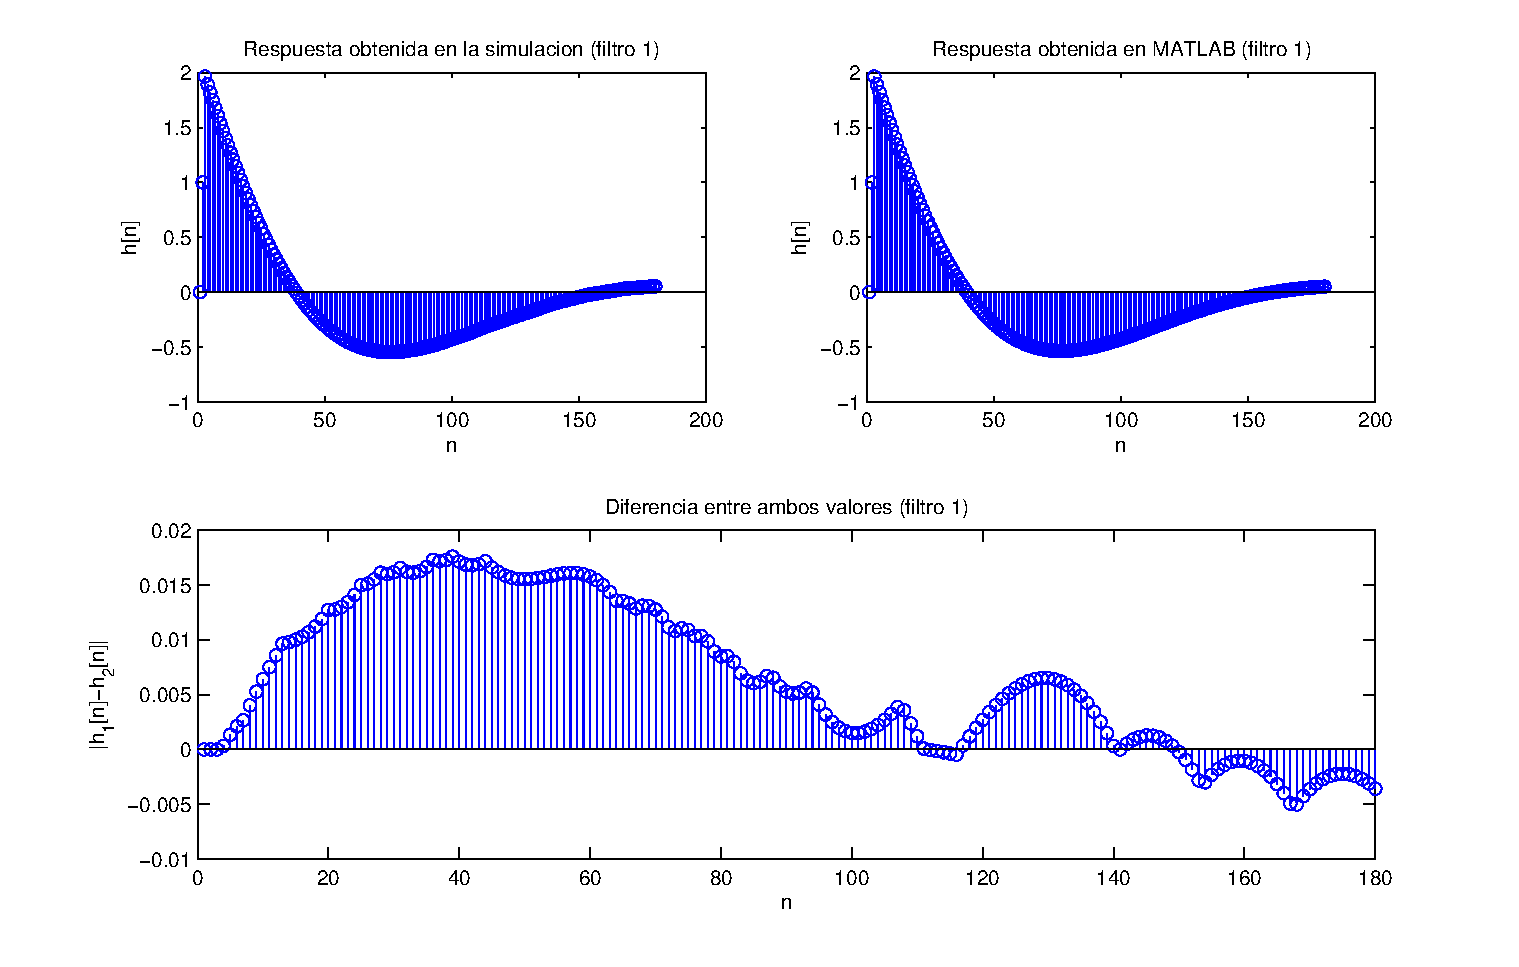
\includegraphics[width=\textwidth]{img/respfiltro1.pdf} 
\caption{Comprobación del filtro 1} \label{fig:filter1}
\end{figure}

\begin{figure}[hbt]
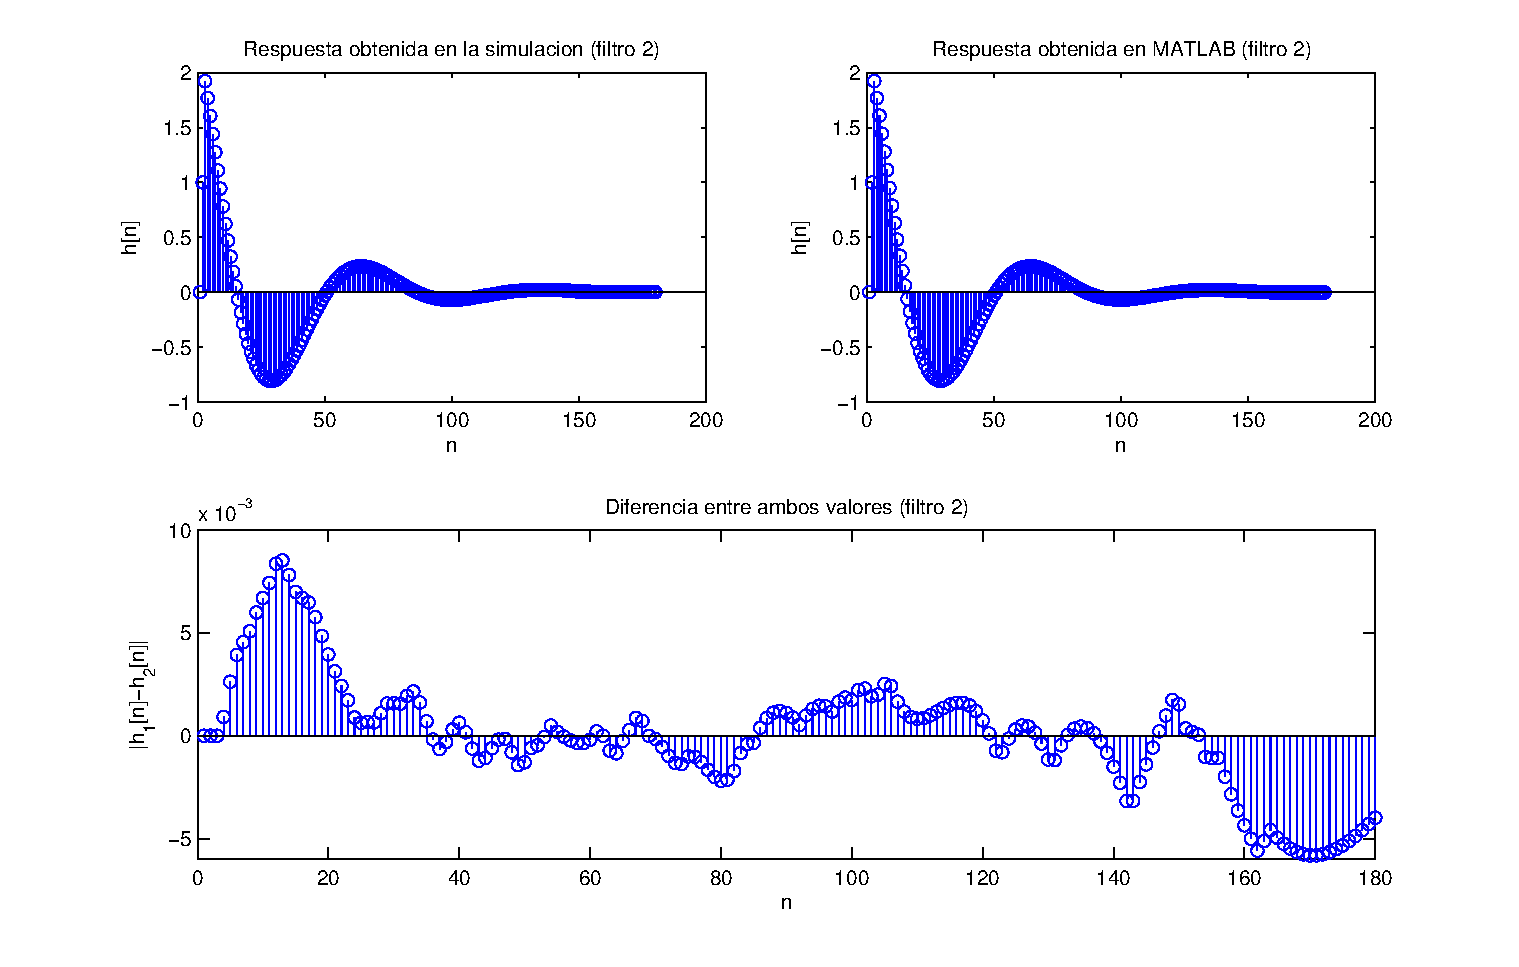
\includegraphics[width=\textwidth]{img/respfiltro2.pdf} 
\caption{Comprobación del filtro 2} \label{fig:filter2}
\end{figure}

\begin{figure}[hbt]
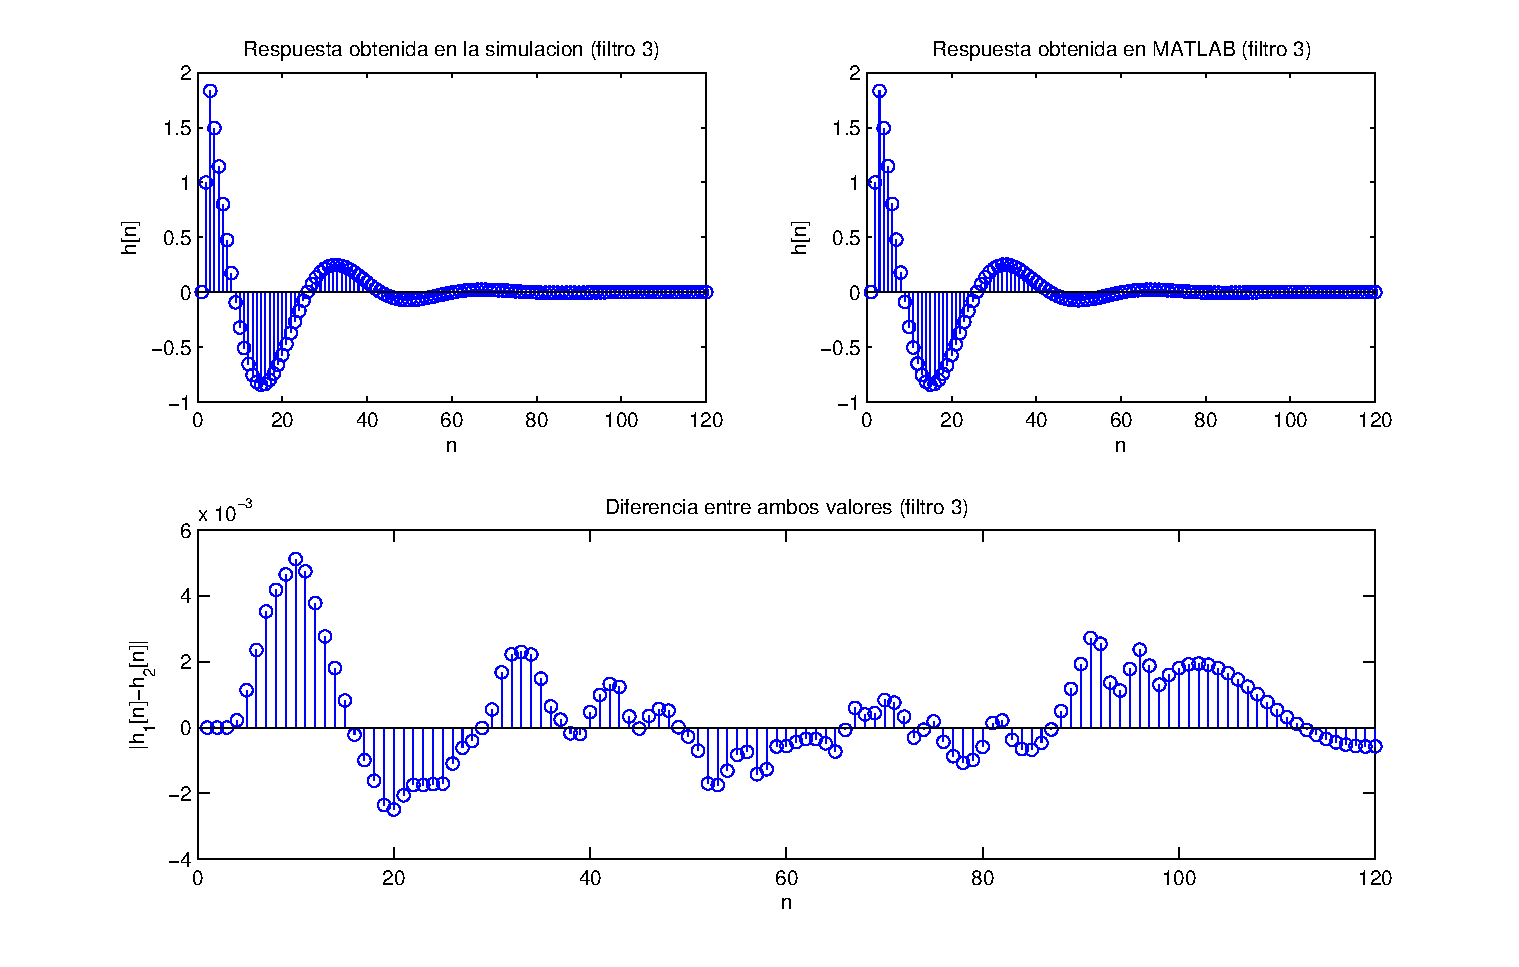
\includegraphics[width=\textwidth]{img/respfiltro3.pdf} 
\caption{Comprobación del filtro 3} \label{fig:filter3}
\end{figure}

\begin{figure}[hbt]
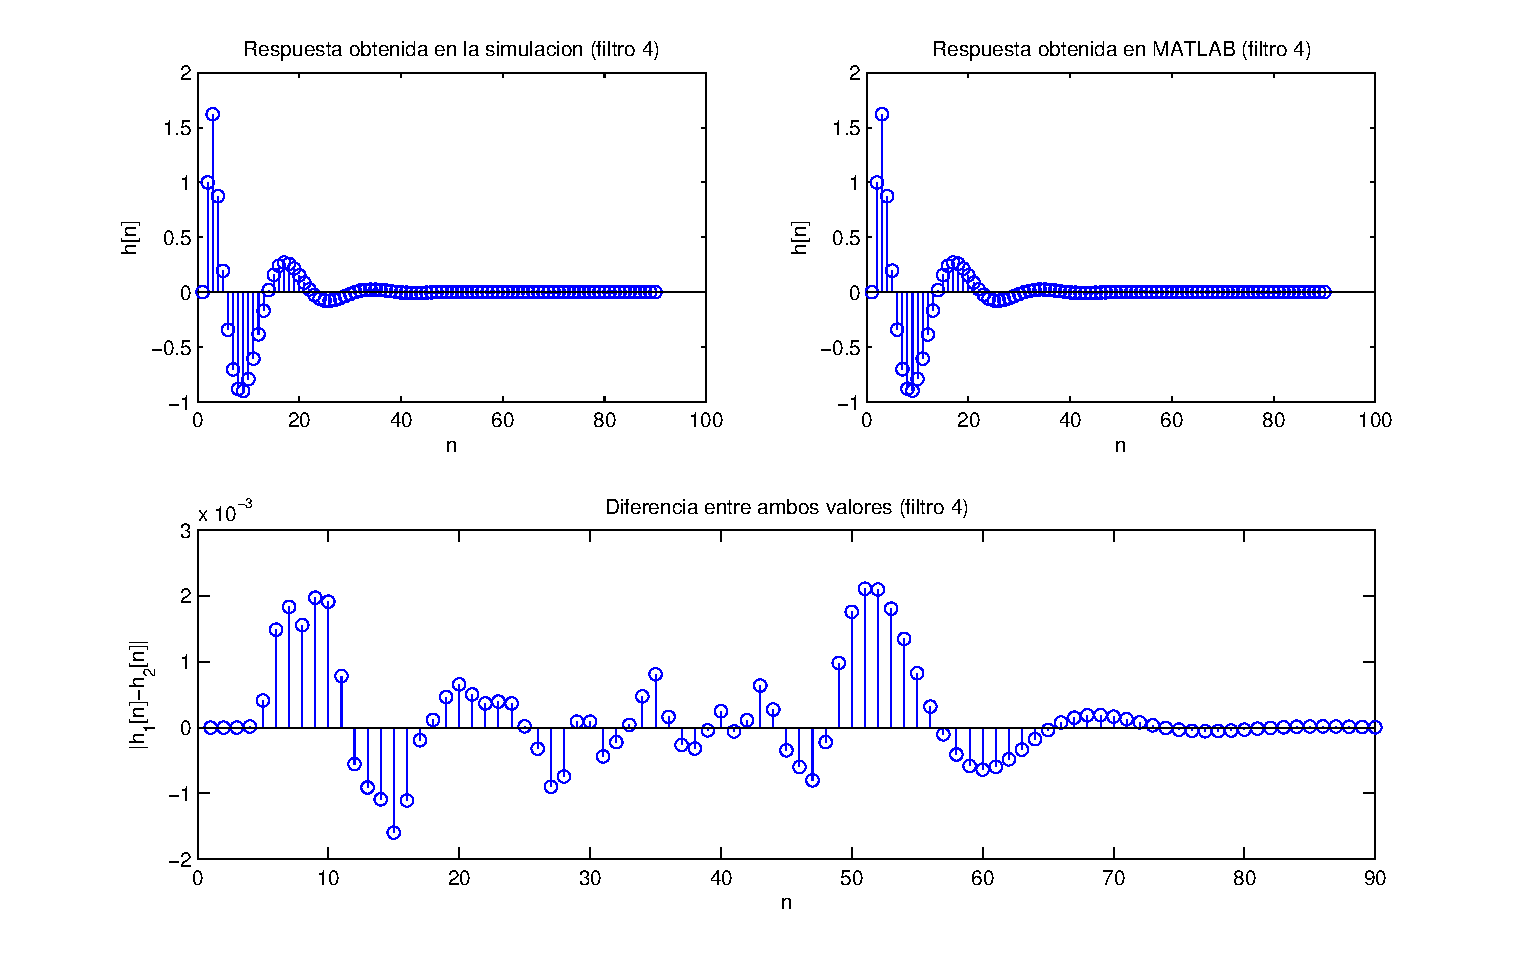
\includegraphics[width=\textwidth]{img/respfiltro4.pdf} 
\caption{Comprobación del filtro 4} \label{fig:filter4}
\end{figure}

\begin{figure}[hbt]
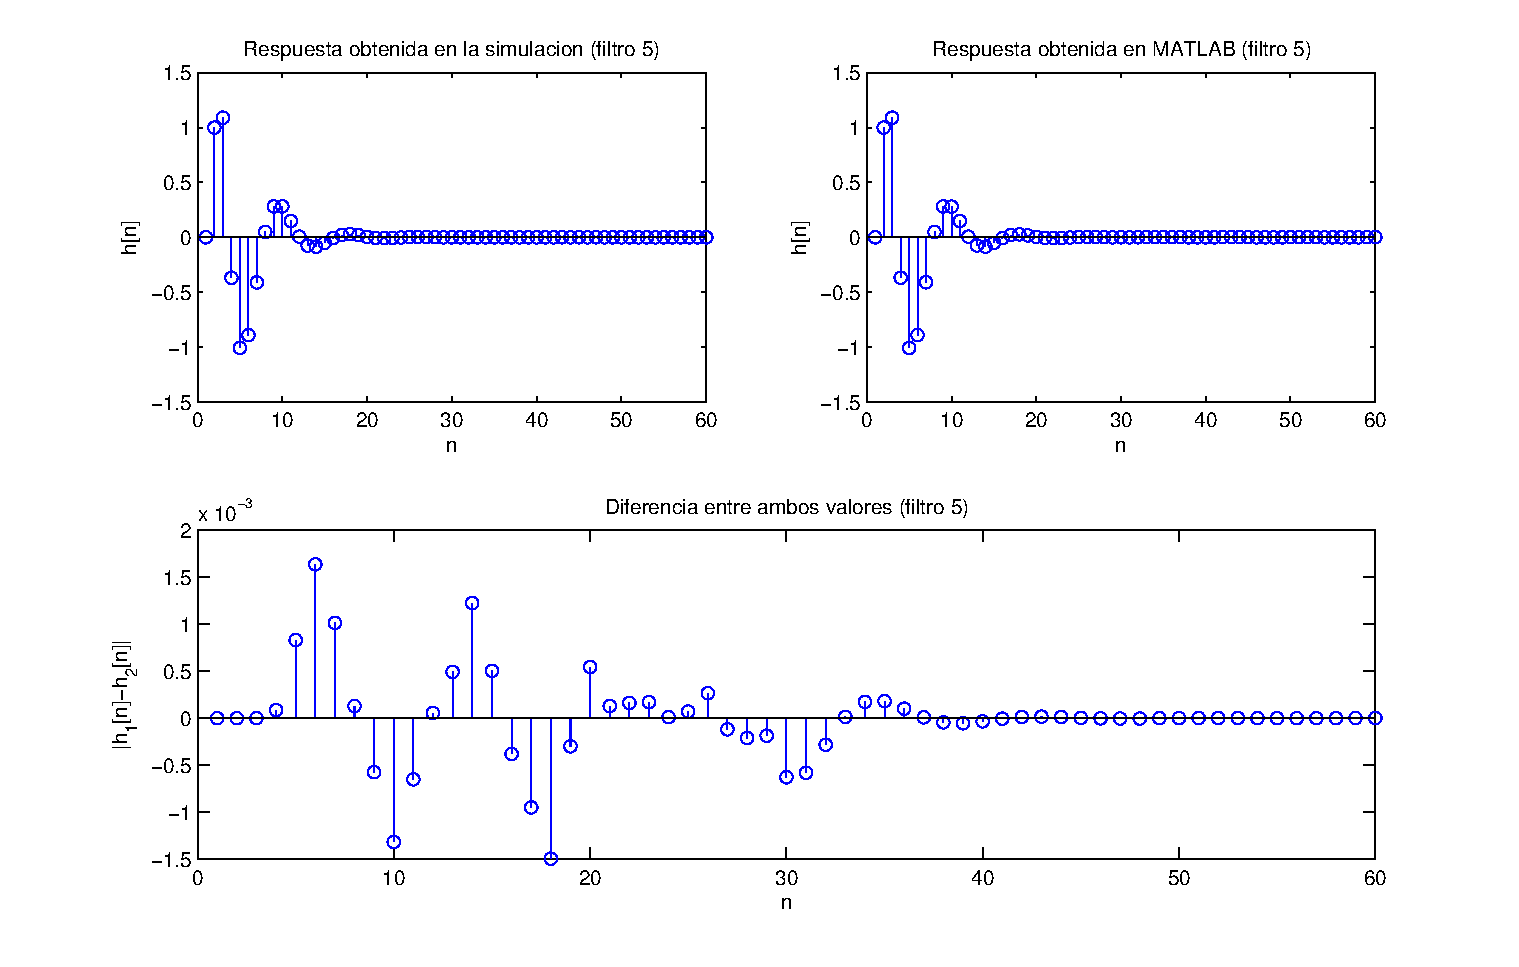
\includegraphics[width=\textwidth]{img/respfiltro5.pdf} 
\caption{Comprobación del filtro 5} \label{fig:filter5}
\end{figure}

\begin{figure}[hbt]
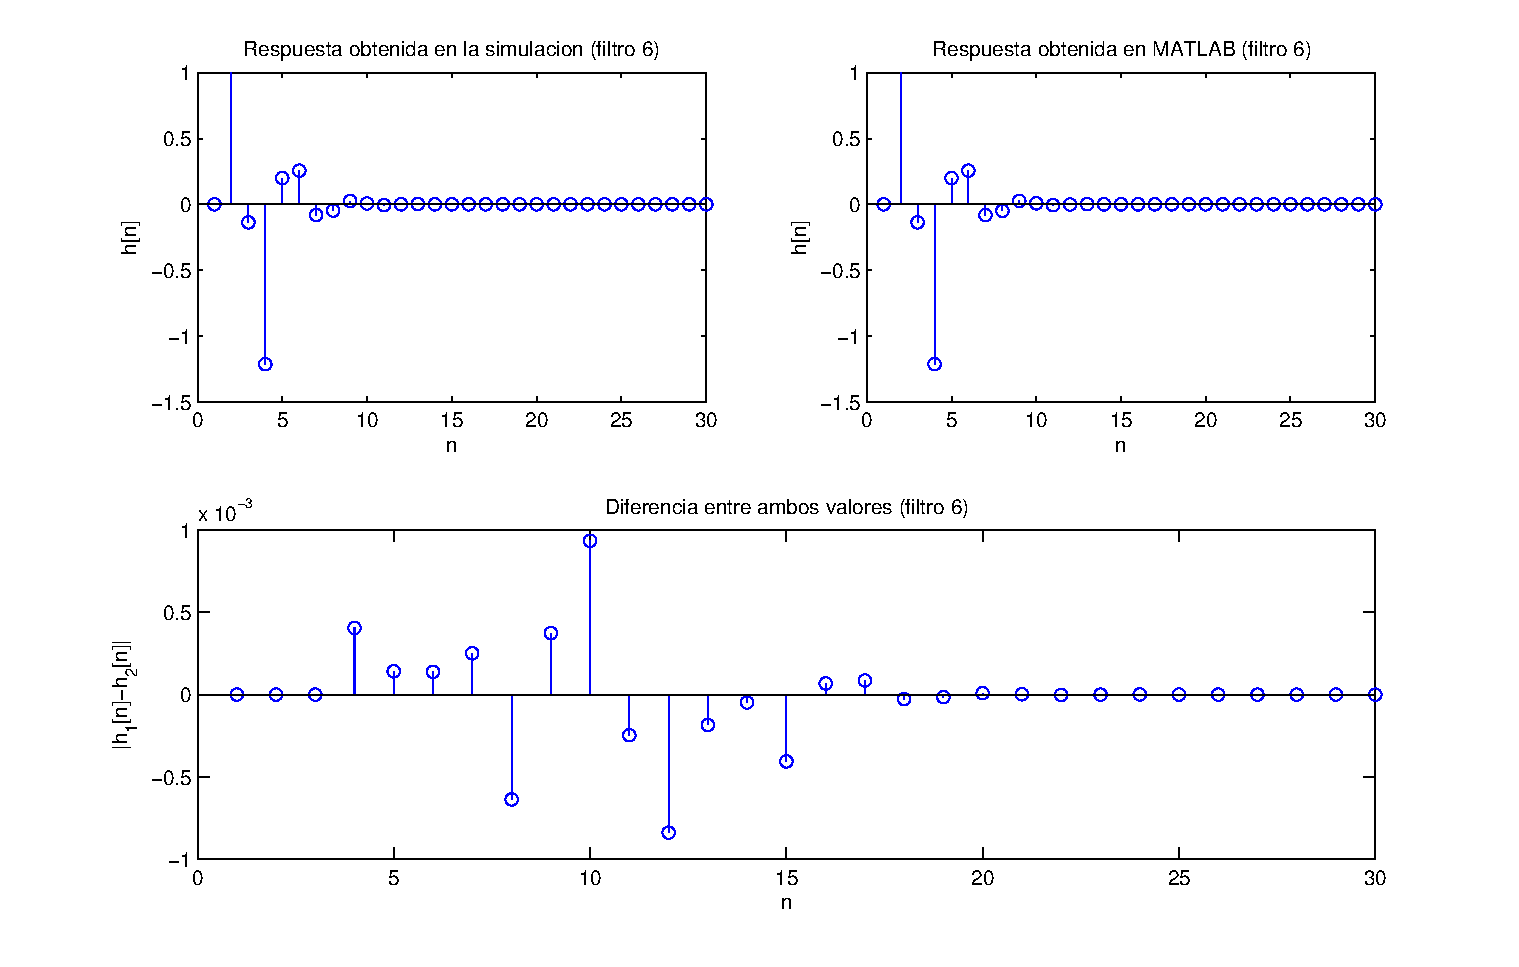
\includegraphics[width=\textwidth]{img/respfiltro6.pdf} 
\caption{Comprobación del filtro 6} \label{fig:filter6}
\end{figure}

\clearpage

\section{Detalle de los programas para la prueba de los filtros}
En esta sección vamos a describir más detalladamente los programas utilizados para comprobar que los filtros se han realizado correctamente.

En concreto, hemos realizado un programa de simulación en ModelSim, donde definimos la señal de entrada al sistema y obtenemos la señal de salida de cada filtro. Esta señal deberá ser posteriormente exportada, y utilizaremos MATLAB para comparar esta señal con la respuesta la impulso que generaría un filtro creado con la función \emph{filter(B,A)} de MATLAB.

A continuación describiremos el procedimiento seguido en ambos programas.

\subsection{Programa ModelSim utilizado para la simulación}

En primer lugar vamos a describir el programa utilizado en ModelSim para la simulación de los filtros anteriormente descritos. Con este fin se ha utilizado un programa de prueba en el que se incluyen los 7 filtros y se estimulan con una señal $\delta[n]$. La salida de los 7 filtros es convertida a un número entero para mayor comodidad.

Los resultados de la simulación se exportaran en forma de lista para ser importados en \emph{MATLAB} y evaluados como hemos visto anteriormente. Es importante tener en cuenta que aunque nosotros estamos exportando números enteros, en nuestra representación de vectores de bits habíamos tomado 6 bits enteros y 10 bits fraccionarios. Como consecuencia, habrá que dividir los valores obtenidos por 1024 antes de poder comparar la respuesta al impulso en MATLAB.

A continuación se muestra el programa VHDL que obtiene la respuesta al impulso de los filtros diseñados.

\begin{vhdlcode}
library ieee;
use ieee.std_logic_1164.all;
use ieee.numeric_std.all;

  

entity test_filter is
    PORT (
             iout0 : out integer;
            iout1 : out integer;
            iout2 : out integer;
            iout3 : out integer;
            iout4 : out integer;
            iout5 : out integer;
            iout6 : out integer);
end;

architecture only of test_filter is

signal sout0 : std_logic_vector (15 downto 0);
signal sout1 : std_logic_vector (15 downto 0);
signal sout2 : std_logic_vector (15 downto 0);
signal sout3 : std_logic_vector (15 downto 0);
signal sout4 : std_logic_vector (15 downto 0);
signal sout5 : std_logic_vector (15 downto 0);
signal sout6 : std_logic_vector (15 downto 0);

signal out0 : signed (15 downto 0);
signal out1 : signed (15 downto 0);
signal out2 : signed (15 downto 0);
signal out3 : signed (15 downto 0);
signal out4 : signed (15 downto 0);
signal out5 : signed (15 downto 0);
signal out6 : signed (15 downto 0);

COMPONENT filter0
    port (
        sin : in std_logic_vector (15 downto 0);
        sout : out std_logic_vector (15 downto 0);
        clk : in bit);
END COMPONENT ;

COMPONENT filter1
    port (
        sin : in std_logic_vector (15 downto 0);
        sout : out std_logic_vector (15 downto 0);
        clk : in bit);
END COMPONENT ;

COMPONENT filter2
    port (
        sin : in std_logic_vector (15 downto 0);
        sout : out std_logic_vector (15 downto 0);
        clk : in bit);
END COMPONENT ;

COMPONENT filter3
    port (
        sin : in std_logic_vector (15 downto 0);
        sout : out std_logic_vector (15 downto 0);
        clk : in bit);
END COMPONENT ;

COMPONENT filter4
    port (
        sin : in std_logic_vector (15 downto 0);
        sout : out std_logic_vector (15 downto 0);
        clk : in bit);
END COMPONENT ;

COMPONENT filter5
    port (
        sin : in std_logic_vector (15 downto 0);
        sout : out std_logic_vector (15 downto 0);
        clk : in bit);
END COMPONENT ;

COMPONENT filter6
    port (
        sin : in std_logic_vector (15 downto 0);
        sout : out std_logic_vector (15 downto 0);
        clk : in bit);
END COMPONENT ;

SIGNAL clk   : bit := '0';
SIGNAL sin  : std_logic_vector (15 downto 0) 
            := "0000000000000000";

begin
out0 <= signed(sout0);
out1 <= signed(sout1);
out2 <= signed(sout2);
out3 <= signed(sout3);
out4 <= signed(sout4);
out5 <= signed(sout5);
out6 <= signed(sout6);

iout0 <= to_integer(out0);
iout1 <= to_integer(out1);
iout2 <= to_integer(out2);
iout3 <= to_integer(out3);
iout4 <= to_integer(out4);
iout5 <= to_integer(out5);
iout6 <= to_integer(out6);

dut0 : filter0 
   PORT MAP (
   sin => sin,
   clk => clk,
   sout => sout0);

dut1 : filter1 
   PORT MAP (
   sin => sin,
   clk => clk,
   sout => sout1);

dut2 : filter2 
   PORT MAP (
   sin => sin,
   clk => clk,
   sout => sout2);

dut3 : filter3 
   PORT MAP (
   sin => sin,
   clk => clk,
   sout => sout3);
   
dut4 : filter4
   PORT MAP (
     sin => sin,
     clk => clk,
     sout => sout4);

dut5 : filter5
   PORT MAP (
   sin => sin,
   clk => clk,
   sout => sout5);

dut6 : filter6 
   PORT MAP (
   sin => sin,
   clk => clk,
   sout => sout6);

clock : PROCESS
   begin
   wait for 10 ns; clk  <= not clk;
end PROCESS clock;

stimulus : PROCESS
   begin
   sin <= "0000000000000000";
   wait for 5 ns; sin  <= "0000010000000000";
   wait for 10 ns; sin  <= "0000000000000000";
   wait;
end PROCESS stimulus;

end only;
\end{vhdlcode}
\clearpage

\subsection{Programa MATLAB utilizado para la comprobación}
Obtener la respuesta al impulso de los filtros en MATLAB es muy sencillo. MATLAB permite crear filtros a partir de sus coeficientes A y B, los mismos que hemos utilizado para la implementación en VHDL. Para obtener la respuesta al impulso simplemente deberemos generar una función $\delta[n]$ y calcular la salida del filtro utilizándola como entrada.

A continuación se muestra el código del programa MATLAB utilizado con este fin.

\emph{NOTA: La respuesta al impulso obtenida en ModelSIM de los filtros implementados, se encuentra en el archivo responses.lst, que será cargado para realizar la comparación.}

\begin{matlabcode}

A = [1024 -2029 1006;
    1024 -2011 988;
    1024 -1970 955;
    1024 -1878 890;
    1024 -1660 772;
    1024 -1115 569;
    1024 141 239];
B = [1024 0 -1024;
    1024 0 -1024;
    1024 0 -1024;
    1024 0 -1024;
    1024 0 -1024;
    1024 0 -1024;
    1024 0 -1024;];



h = dlmread('responses.lst');
h = h ./ 1024;
for i = 1:7,
    delta = zeros(1,200);
    delta(2) = 1;
    hi = transpose(h(:,i))
    Bi = B(i,:)
    Ai = A(i,:)
    yi = filter(Bi, Ai, delta)
    diff = yi-hi;
    subplot(2,2,1); stem(hi);
    title('Respuesta obtenida en la simulacion')
    xlabel('n')
    ylabel('h[n]')
    subplot(2,2,2); stem(yi);
    title('Respuesta obtenida en MATLAB')
    xlabel('n')
    ylabel('h[n]')
    subplot(2,2,[3:4]); stem(diff);
    title('Diferencia entre ambas respuestas')
    xlabel('n')
    ylabel('|h_1[n]-h_2[n]|')
    pause
    subplot
end

\end{matlabcode}
\clearpage

\end{document}













